\graphicspath{{./img}} % path to graphics

\section*{\LARGE Введение}
\addcontentsline{toc}{section}{Введение}
Направление связи состоит из двух каналов (основного и
резервного) и общего входного буфера емкостью на Еmk
сообщений.\par
На направление поступают два потока сообщений с
экспоненциально распределенными интервалами времени, средние
значения которых Т1 = 3 мин и Т2 = 4 мин. При нормальной
работе сообщения передаются по основному каналу. Время
передачи одного сообщения распределено по экспоненциальному
закону со средним значением Т3 = 2 мин.\par
В основном канале происходят сбои через интервалы времени,
распределенные по экспоненциальному закону со средним
значением Т4 = 15 мин. Если сбой происходит во время передачи,
то сообщение теряется. За время Т5 = 5 с запускается резервный
канал, который передает сообщения, начиная с очередного. Время
передачи одного сообщения распределено по экспоненциальному
закону со средним значением Т6 = 3 мин.\par
Основной канал восстанавливается. Время восстановления
канала подчинено экспоненциальному закону со средним
значением Т7 = 2 мин. После восстановления резервный канал
выключается и основной канал продолжает работу с очередного
сообщения.\par
Необходимо разработать имитационную модель и провести
исследование функционирования направления связи в течение 2 ч.\par
Определить:
\begin{itemize}
	\item рациональную емкость накопителя;
	\item загрузку основного и резервного каналов связи;
	\item вероятности передачи сообщений потока 1 и потока 2;
	\item вероятность передачи сообщений направлением связи в целом. 
\end{itemize}

\clearpage

\section*{\LARGE Выполнение практической работы}
\addcontentsline{toc}{section}{Выполнение практической работы}
Запустим модель и проанализируем работу системНаправление связи
представляет собой систему массового обслуживания разомкнутого типа с
ожиданием и с отказами из-за ограниченной ёмкости входного буфера. А также
с выходами из строя (временного не функционирования) основного канала.\par
В модели сообщения следует представлять заявками, основной
и резервный канал — одноканальными устройствами (ОКУ), 
входной буфер (накопитель) — очередью. В очереди следует
использовать дисциплину обслуживания FIFO.\par
Введём масштабирование: 1 единица модельного времени
соответствует 1 с, то есть, например, время моделирования равно 2
часам, тогда 2*60*60 = 7200 единиц модельного времени.
Аналогично Т1 = 120, Т2 =240 и т.д.\par
Декомпозиция системы и состав сегментов модели
определяются разработчиком. Введём в модели
функционирования направления связи следующие сегменты:

\begin{itemize}
	\item исходные данные;
	\item источники сообщений;
	\item буфер, основной и резервный каналы связи;
	\item имитатор отказов основного канала;
	\item результаты моделирования.
\end{itemize}

Итоговая модель проиллюстрированна на рисунке~\ref{fig:model:res}.

\begin{image}
	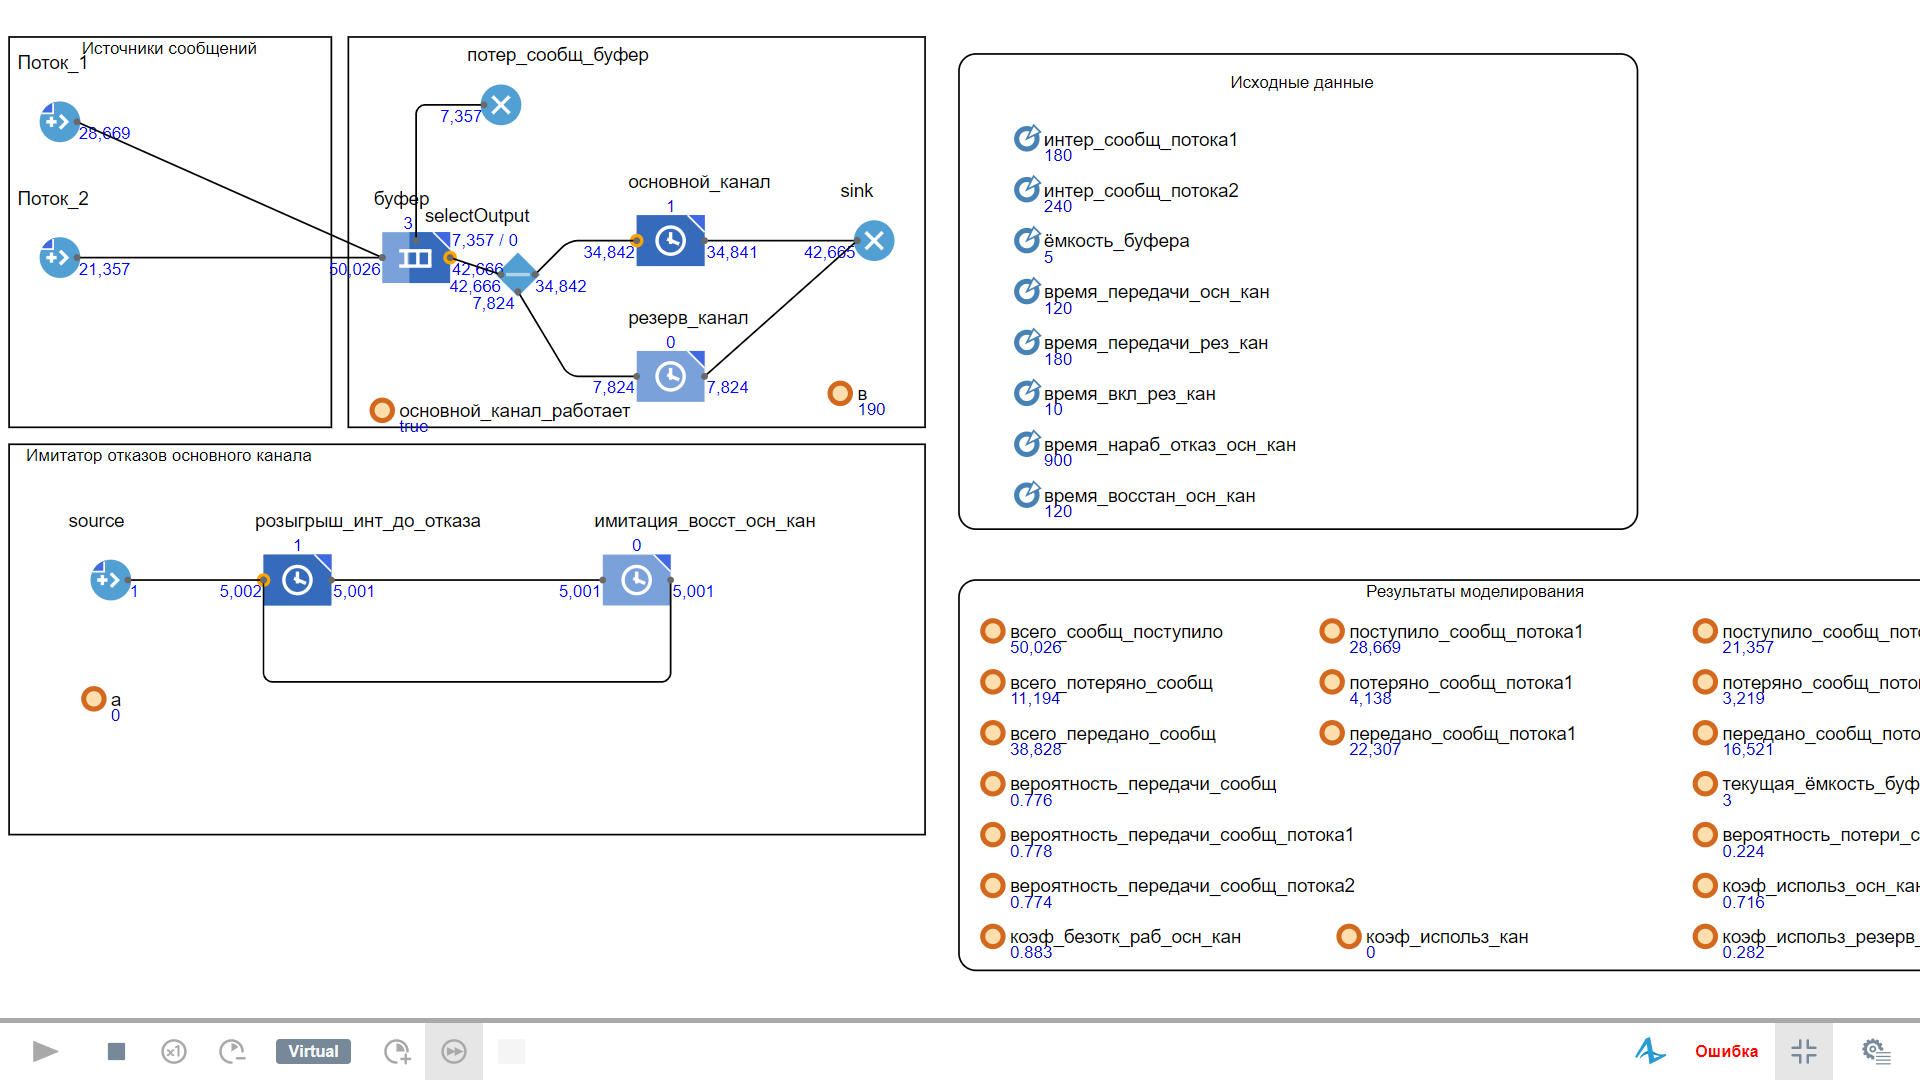
\includegraphics[width=1\textwidth]{png1}
	\caption{Модель направления связи}
	\label{fig:model:res}
\end{image}

\clearpage

\section*{\LARGE Вывод}
\addcontentsline{toc}{section}{Вывод}
В данной практической работе была создана модель направления связей
состоящей из двух каналов (основного и резервного) и общего входного
буфера емкостью на Еmk сообщений.

\begin{longtable} {
	|p{0.45\textwidth}
	|p{0.1\textwidth}
	|p{0.13\textwidth}
	|p{0.13\textwidth}
	|p{0.13\textwidth}
	|}
	\caption{\leftline{Показатели функционирования направления связи}}\\
	\hline Показатели & GPSS World & AnyLogic6
		& AnyLogic7 & AnyLogic8 \\ \hline
	\endhead

	\multicolumn{5}{|c|}{1) объем\_буфера = 5} \\ \hline
	вероятность\_передачи\_сообщ & 0,752 & 0,773 & 0,773 & 0.776 \\ \hline
	вероятность\_передачи\_сообщ \_потока1 & 0,752 & 0,772
		& 0,771 & 0.778\\ \hline
	вероятность\_передачи\_сообщ \_потока2 & 0,753 & 0,773
		& 0,774 & 0.774\\ \hline
	$\delta$1 вероятности\_передачи\_сообщ &
		\multicolumn{4}{|c|}{$\delta$1 = 0,021} \\ \hline
	вероятность \_потери\_сообщ & 0,248 & 0,227 & 0,227 & 0.224 \\ \hline
	коэф\_использ \_осн\_кан & 0,777 & 0,757 & 0,718 & 0.716 \\ \hline
	коэф\_использ \_рез\_кан & 0,152 & 0,222 & 0,286 & 0.282 \\ \hline
	сум\_коэф \_использ\_кан & 0,929 & 0,979 & 1,003 & 0.998 \\ \hline
	\multicolumn{5}{|c|}{2) объем\_буфера = 10} \\ \hline
	вероятность\_передачи\_сообщ & 0,829 & 0,861 & 0,831 & 0.838 \\ \hline
	вероятность\_передачи\_сообщ \_потока1 & 0,829 & 0,861
		& 0,832 & 0.839\\ \hline
	вероятность\_передачи\_сообщ \_потока2 & 0,829 & 0,862
		& 0,831 & 0.837 \\ \hline
	$\delta$2 вероятности\_передачи\_сообщ &
		\multicolumn{4}{|c|}{$\delta$2 =0,002} \\ \hline
	вероятность\_потери\_сообщ & 0,171 & 0,139 & 0,169 & 0.162 \\ \hline
	коэф\_использ\_осн\_кан & 0,861 & 0,841 & 0,756 & 0.757 \\ \hline
	коэф\_использ\_рез\_кан & 0,157 & 0,250 & 0,327 & 0.32 \\ \hline
	сум\_коэф\_использ\_кан & 1,018 & 1,091 & 1,084 & 1.077 \\ \hline
	\multicolumn{5}{|c|}{3) интер\_сообщ\_потока1 = 90,
		интер\_сообщ\_потока2 = 120} \\ \hline
	вероятность\_передачи\_сообщ & 0,438 & 0,454 & 0,456 & 0.461 \\ \hline
	вероятность\_передачи\_сообщ \_потока1 & 0,438 & 0,454
		& 0,456 & 0.463 \\ \hline
	вероятность\_передачи\_сообщ \_потока2 & 0,438 & 0,453
		& 0,456 & 0.459 \\ \hline
	$\delta$3 вероятности\_передачи\_сообщ &
		\multicolumn{4}{|c|}{$\delta$3 = 0,002} \\ \hline
	вероятность\_потери\_сообщ & 0,562 & 0,546 & 0,544 & 0.539 \\ \hline
	коэф\_использ\_осн\_кан & 0,882 & 0,882 & 0,808 & 0.813 \\ \hline
	коэф\_использ\_рез\_кан & 0,209 & 0,266 & 0,393 & 0.387 \\ \hline
	сум\_коэф\_использ\_кан & 1,091 & 1,148 & 1,201 & 1.2 \\ \hline
	\multicolumn{5}{|c|}{4) время\_передачи\_осн\_кан = 60,
		время\_нараб\_отказ\_осн\_кан = 5000} \\ \hline
	вероятность\_передачи\_сообщ & 0,844 & 0,848 & 0,815 & 0.819 \\ \hline
	вероятность\_передачи\_сообщ \_потока1 & 0,844 & 0,848
		& 0,815 & 0.821 \\ \hline
	вероятность\_передачи\_сообщ \_потока2 & 0,845 & 0,848
		& 0,815 & 0.816 \\ \hline
	$\delta$4 вероятности\_передачи\_сообщ &
		\multicolumn{4}{|c|}{$\delta$4 = 0,029} \\ \hline
	вероятность\_потери\_сообщ & 0,156 & 0,152 & 0,185 & 0.181 \\ \hline
	коэф\_использ\_осн\_кан & 0,971 & 0,970 & 0,922 & 0.921 \\ \hline
	коэф\_использ\_рез\_кан & 0,043 & 0,058 & 0,088 & 0.089 \\ \hline
	сум\_коэф\_использ\_кан & 1,014 & 1,028 & 1,010 & 1.01 \\ \hline
	\multicolumn{5}{|c|}{5) время\_передачи\_рез\_кан = 90,
		время\_восстан\_осн\_кан = 60} \\ \hline
	вероятность\_передачи\_сообщ & 0,851 & 0,857 & 0,834 & 0.836 \\ \hline
	вероятность\_передачи\_сообщ \_потока1 & 0,851 & 0,857
		& 0,833 & 0.838 \\ \hline
	вероятность\_передачи\_сообщ \_потока2 & 0,851 & 0,857
		& 0,835 & 0.833 \\ \hline
	$\delta$5 вероятности\_передачи\_сообщ &
		\multicolumn{4}{|c|}{$\delta$5 = 0,017} \\ \hline
	вероятность\_потери\_сообщ & 0,149 & 0,143 & 0,166 & 0.164 \\ \hline
	коэф\_использ\_осн\_кан & 0,982 & 0,980 & 0,945 & 0.947 \\ \hline
	коэф\_использ\_рез\_кан & 0,017 & 0,029 & 0,043 & 0.041 \\ \hline
	сум\_коэф\_использ\_кан & 0,999 & 1,009 & 0,988 & 0.989 \\ \hline
	\multicolumn{5}{|c|}{6) интер\_сообщ\_потока1 = 45,
		интер\_сообщ\_потока2 = 60} \\ \hline
	вероятность\_передачи\_сообщ & 0,430 & 0,432 & 0,434 & 0.434 \\ \hline
	вероятность\_передачи\_сообщ \_потока1 & 0,431 & 0,432
		& 0,434 & 0.433 \\ \hline
	вероятность\_передачи\_сообщ \_потока2 & 0,429 & 0,431
		& 0,434 & 0.436 \\ \hline
	$\delta$6 вероятности\_передачи\_сообщ &
		\multicolumn{4}{|c|}{$\delta$6 = 0,004} \\ \hline
	вероятность\_потери\_сообщ & 0,570 & 0,568 & 0,566 & 0.566 \\ \hline
	коэф\_использ\_осн\_кан & 0,988 & 0,988 & 0,980 & 0.981 \\ \hline
	коэф\_использ\_рез\_кан & 0,024 & 0,029 & 0,048 & 0.043 \\ \hline
	сум\_коэф\_использ\_кан & 1,012 & 1,017 & 1,028 & 1.024 \\ \hline
	\multicolumn{5}{|c|}{7) время\_передачи\_осн\_кан = 30,
		время\_передачи\_рез\_кан = 45} \\ \hline
	вероятность\_передачи\_сообщ & 0,850 & 0,853 & 0,832 & 0.83 \\ \hline
	вероятность\_передачи\_сообщ \_потока1 & 0,851 & 0,853
		& 0,831 & 0.832 \\ \hline
	вероятность\_передачи\_сообщ \_потока2 & 0,850 & 0,853
		& 0,832 & 0.828 \\ \hline
	$\delta$7 вероятности\_передачи\_сообщ &
		\multicolumn{4}{|c|}{$\delta$7 = 0,018} \\ \hline
	вероятность\_потери\_сообщ & 0,150 & 0,147 & 0,168 & 0.17 \\ \hline
	коэф\_использ\_осн\_кан & 0,982 & 0,982 & 0,952 & 0.955 \\ \hline
	коэф\_использ\_рез\_кан & 0,015 & 0,021 & 0,028 & 0.026 \\ \hline
	сум\_коэф\_использ\_кан & 0,997 & 1,003 & 0,980 & 0.981 \\ \hline
	\multicolumn{5}{|c|}{8) время\_вкл\_рез\_кан = 1,
		время\_восстан\_осн\_кан = 30}  \\ \hline
	вероятность\_передачи\_сообщ & 0,851 & 0,855 & 0,833 & 0.826 \\ \hline
	вероятность\_передачи\_сообщ \_потока1 & 0,851 & 0,855
		& 0,833 & 0.825 \\ \hline
	вероятность\_передачи\_сообщ \_потока2 & 0,851 & 0,855
		& 0,832 & 0.827 \\ \hline
	$\delta$8 вероятности\_передачи\_сообщ &
		\multicolumn{4}{|c|}{$\delta$8 = 0,018} \\ \hline
	вероятность\_потери\_сообщ & 0,149 & 0,145 & 0,167 & 0.174 \\ \hline
	коэф\_использ\_осн\_кан & 0,988 & 0,987 & 0,957 & 0.958 \\ \hline
	коэф\_использ\_рез\_кан & 0,008 & 0,015 & 0,021 & 0.023 \\ \hline
	сум\_коэф\_использ\_кан & 0,996 & 1,002 & 0,978 & 0.981 \\ \hline

\end{longtable}

